% !Mode:: "TeX:UTF-8"

\chapter[基于计算机视觉和深度学习的结构健康监测异常数据诊断]{基于计算机视觉和深度学习的结构健康监测\protect\\异常数据诊断}[Computer Vision and Deep Learning-based Data Anomaly Detection Method for Structural Health Monitoring]

近年来,结构健康监测(Structural Health Monitoring, SHM)系统在土木基础设施中广泛应用,产生了大量的数据。结构健康监测数据的分析和挖掘已成为土木工程领域的研究热点。然而,由于土木结构的服役恶劣环境,结构健康监测系统测量的数据受到多种异常数据的污染,严重影响了数据分析结果。同时,这也是实现自动实时预警的主要障碍之一,因为很难区分结构破坏造成的异常和与错误数据导致的异常。现有的数据清洗方法主要针对去噪,而错误数据的检测需要领域专业知识,人力、时间成本高昂。受现实世界人工检测过程的启发,本章提出了一种基于计算机视觉和深度学习的数据异常检测方法。方法框架包括两个步骤:通过数据可视化进行数据转换,以及构建和训练深度神经网络(Deep Neural Networks, DNNs)进行异常分类。这个过程模仿了人类的生物视觉和逻辑思考过程。在第一步中,首先将时间序列信号分段可视化为灰度图像,然后转化为图像向量,。在第二步中,由随机选择的手动标记的图像向量组成的训练数据集被输入到一个DNN或一个DNN集群中,通过堆栈式自动编码器(stacked autoencoders)和逐层贪婪训练方法(greedy layer-wise training)对其进行训练。训练后的DNN可用于检测大量未经检查的结构健康监测数据中的潜在异常。采用了中国某座大跨度斜拉桥结构健康监测系统的加速度数据验证了方法可行性和性能。结果表明,本方法可以快速、自动、准确地完成多类别的异常数据诊断。

本章的内容顺序如下:

\section{基于计算机视觉和深度学习的异常数据诊断方法框架}[Framework of the computer vision and deep learning-based data anomaly detection method]

所提出的方法框架包括两个主要步骤,如图1所示:(1)通过数据可视化进行数据转换;(2)对数据异常分类进行DNN训练。该过程模仿了人类的生物视觉和逻辑思维。在数据可视化步骤中,将时间序列信号分成若干部分转化为图像向量,并绘制成灰度图像。在第二步中,由随机选择和手动标记的图像向量组成的训练集被输入到DNNs中,然后通过称为堆栈式自动编码器和贪婪的层明智训练的技术对其进行训练。训练后的DNNs可以检测大量SHM数据中的潜在异常。

\begin{figure}[!h]
\centering\includegraphics[trim=3cm 0cm 3cm 0cm, width=0.9\textwidth]{fig_3-1.pdf}
\vspace{0.2em}
\bicaption[Donation]{}{基于计算机视觉和深度学习的异常数据诊断方法框架}{Fig.$\!$}{Framework of the proposed data anomaly detection method}
\end{figure}

\subsection{数据可视化}[Data visualization]
% \subsubsection{摘要}[Abstraction]

为了像人类专家一样自动检测SHM数据中的多个异常点,第一步是数据可视化。将原始数据分割成一个小时的片段,然后用数字绘制并保存为图像文件,如图1所示。拆分数据可以看作是窗口化数据,相邻两个窗口之间没有重叠。每幅图像的像素分辨率为8位灰度,在保证合理低存储要求的前提下,足以体现数据的图形特征。在这样的分辨率下,每个图像文件的大小小于2 KB,因此每年一个通道的总文件大小约为17 MB。通过像素列的顺序连接组装而成的图像向量是神经网络的输入。数据可视化过程可以看作是一个特征选择过程。

\subsubsection{关键词}[Keywords]
关键词是供检索用的主题词条。关键词应集中体现论文特色,反映研究成果的内涵,具有语
义性,在论文中有明确的出处,并应尽量采用《汉语主题词表》或各专业主题词表提供的规
范词,应列取3$\sim$6个关键词,按词条的外延层次从大到小排列。

\subsection{有监督训练和特征提取}[Supervised training and feature extraction]
\subsubsection{数据标记}[Data labeling]

由于所提出的方法是像人类专家那样通过 "观察 "数字来评价数据质量,因此每幅图像的图形特征是关键点,并选择它们作为分类的标准。然而,SHM系统中的数据异常因结构、传感器类型和放置位置的不同而不同。为了事先获得一定结构的标签知识,如每个异常模式的形式和模式的总数,需要人类专家观察采集数据的图像。

接下来,随机选取标记的训练样本,并手动标记异常模式的索引。这些数据表示为 ,其中为第th个数据片段,是对应的异常模式指数。一般来说,1-5\%的训练配比足以覆盖所有具有代表性的数据异常模式。本文采用单标签分类方法,即当一幅图像出现多个异常特征时,按该图像中所有数据的主要内在特征确定标签。

\subsubsection{深度神经网络构建与训练}[Construction and training of deep neural networks]

人类视觉和计算机视觉的图像获取过程是不同的。在三维空间中,人类是一次性观看图像的全貌,而计算机则是通过连续扫描图像的像素列来 "看 "图像。因此,要向计算机显示图像,就要将图像像素列依次堆叠转化为图像矢量。

为了模仿人类的决策过程,以深刻理解异常的特征,采用了快速有效的Stacked Autoencoder Deep Neural Network.35 DNN是一种具有多个隐藏层的人工神经网络(ANN),它们可以学习输入的高级抽象。20世纪90年代末,由于DNN的训练时间明显偏长,基本被机器学习界所抛弃。2006年,通过引入一种无监督的层-明智的预训练程序,取得了突破性的进展,这使得在短时间内用未标记的数据训练一个深度架构成为可能.36预训练层的堆叠克服了权重调整的消失梯度.35,37。

\begin{figure}[!h]
\centering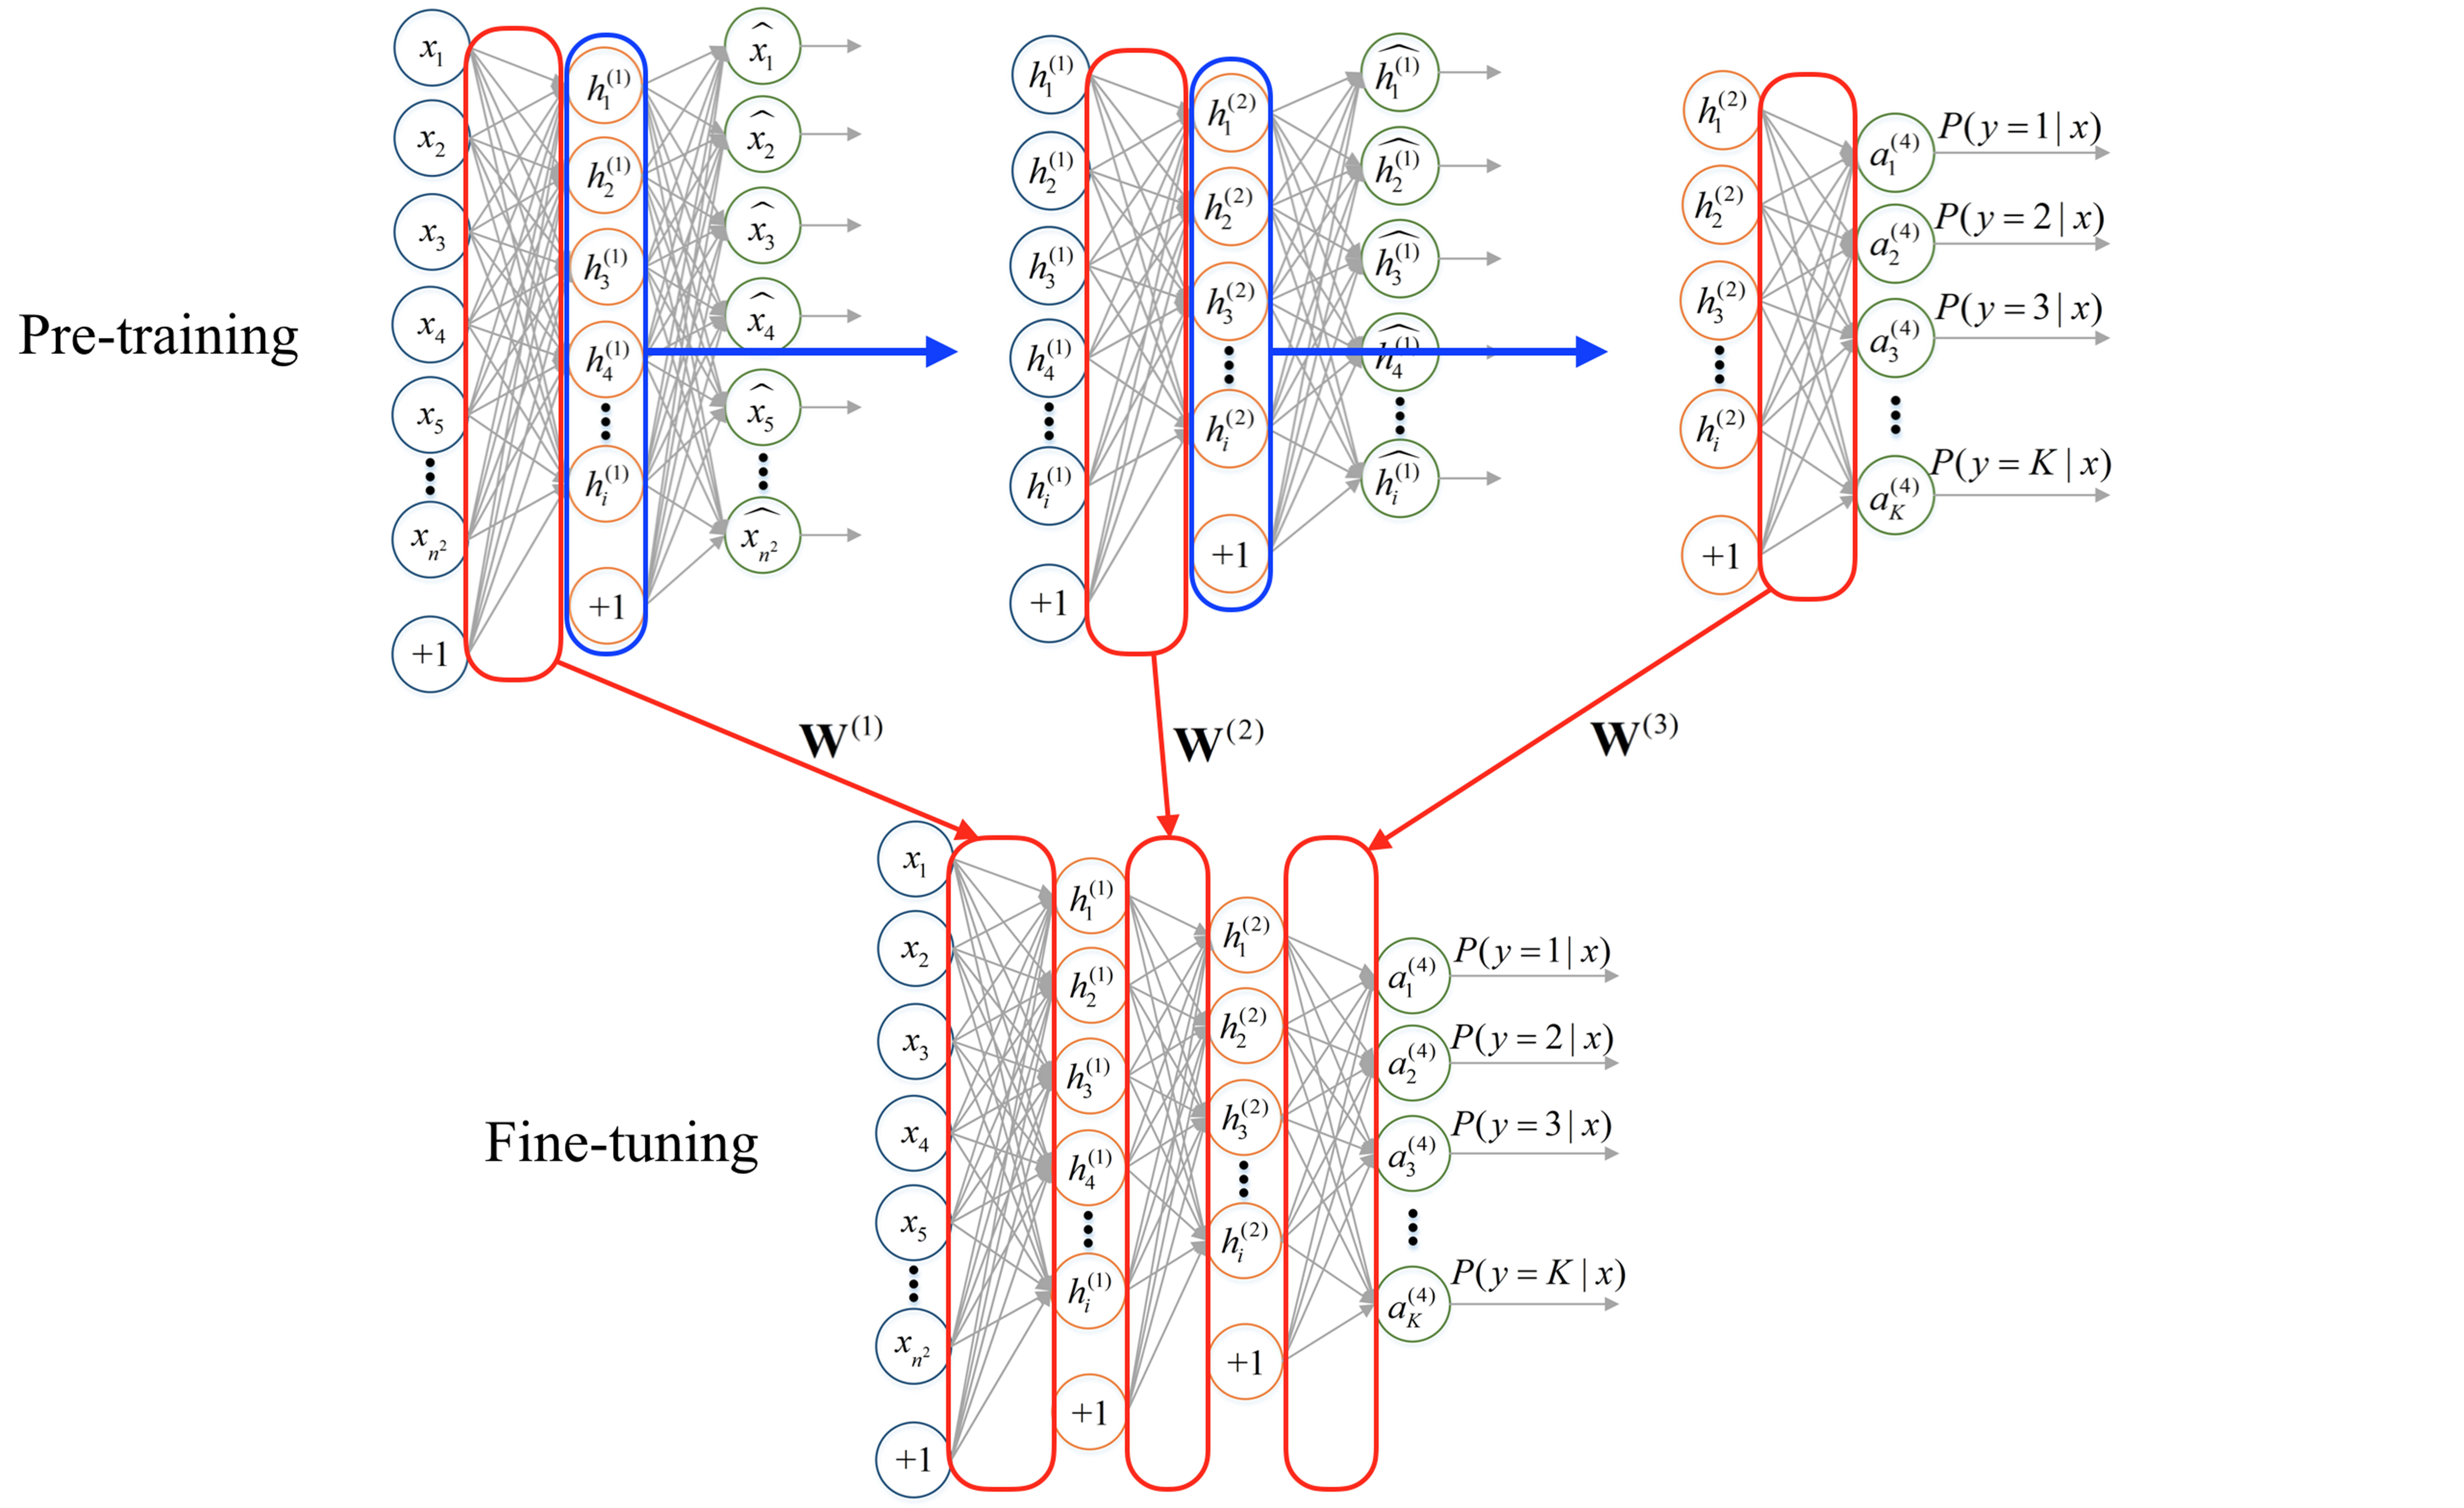
\includegraphics[width=0.9\textwidth]{fig_3-2}
\vspace{0.2em}
\bicaption[Donation]{}{基于计算机视觉和深度学习的异常数据诊断方法框架}{Fig.$\!$}{Framework of the proposed data anomaly detection method}
\end{figure}

构建了一个双隐藏层叠加的自动编码器神经网络来演示两阶段的训练过程。让表示总共数据片中的第th片源数据,表示采样频率,表示每个图中数据的持续时间。因此,每个的采样点数量为 。 若图像像素阵列的维度为 ,则对应的图像向量的维度为 ,如图3所示。

一般来说,在神经网络中,每个单元都有一个激活值,定义为

其中,是层中单元激活的一般符号;在输入层中, ,而在隐藏层中,.是层中单元的输入值;是层的大小;是与层中单元和层中单元之间的联系相关的权重;是与层中单元相关的偏置,它作为多项式中的常数项,是激活函数。

为了简明扼要的记述,矢量化采用元素化的方式。


自动编码器是一个输入层和输出层大小相同的三层ANN,其中输出值被设置为等于输入。因此,自动编码器的训练是无监督的。本文采用sigmoid函数作为隐藏层和输出层的激活函数。



构建双隐藏层堆叠式自动编码器神经网络的第一阶段是贪婪的层间预训练。将图像向量输入到第一个自动编码器中,设定平均方差(MSE)作为目标函数,采用标度共轭梯度(SCG)算法38来调整权重。训练完成后,提取输入层和隐藏层之间的权重,部署到四层神经网络中,为 。每个训练样本的隐藏层的节点值, ,被输入到第二个自动编码器中。训练完成后,提取输入层和第二自动编码器的隐藏层之间的权值,为 。每个自动编码器的输出值是没有用的。最后,在前期训练中,并将每个训练样本的对应标签输入到softmax分类器中,该分类器能够进行多类分类。softmax分类器中输出层的激活函数定义为

其中,是K维的输出向量;是输入列向量;是某类的预测概率 ,因此, ; 是输入层所有单元与输出层第th个单元之间联系的权重行向量;是权重矩阵


接下来,利用交叉熵作为目标函数来衡量实际标签和预测类之间的误差。它被定义为


其中,为目标函数;为样本数;为指标函数,其中和;为样本的类概率 ,即;和为样本的标签。


代入本训练过程中的符号,softmax分类器的激活函数和目标函数分别给出为

其中表示行中的权重向量,表示训练样本的 。

可以通过使用SCG调谐最小化目标函数来获得。因此,通过一个输入层、两个隐藏层和一个softmax层的有序堆叠,使用与自动编码器相同的激活函数,构建一个四层神经网络。需要注意的是,初始权重设置为 ,而不是随机生成。

第二阶段是微调。组成的训练集被输入到使用SCG调优来训练大网络。使用在预训练过程中获得的初始权重可以保证快速收敛35,37。

训练有素的DNN的部署是灵活的,这取决于SHM系统的结构。大规模民用基础设施的SHM系统通常由多个子网组成,每个子网包含多种传感器类型的许多节点。子系统发生的故障会使同一子网中的节点共享同源数据异常模式,如每个传感器的异常数据模式总数和每个模式的图形特征。此外,某一特定的数据异常模式在不同的传感器和不同的子系统中会有不同的出现。因此,为了获得更好的分类性能,最好在训练前为网络设计一个合适的布局。本文提出了三种DNN的网络布局策略。分别是并行布局、融合布局和多组布局,如图3所示。在并行布局中,每个通道都有一个私有网络来检测其数据异常。这种布局具有较好的本地性能,但无法在传感器之间共享信息。相比之下,融合布局将所有传感器的数据混合起来,训练一个全局网络。多组布局结合了上述两种布局,即同一组中的所有传感器共享一个网络,该网络由其融合数据集进行训练。如果SHM系统的传感器子系统结构信息已知,则可以根据实际的传感器子系统结构将传感器分为不同的组,采用多组布局。如果传感器子系统结构信息未知,则应根据各传感器之间同一异常类别的相似性来选择DNN布局。当不同传感器之间同一类异常差异巨大时,适合采用并行布局;如果不同传感器之间每一类异常相似,则采用融合布局更为实用。

\begin{figure}[!h]
\centering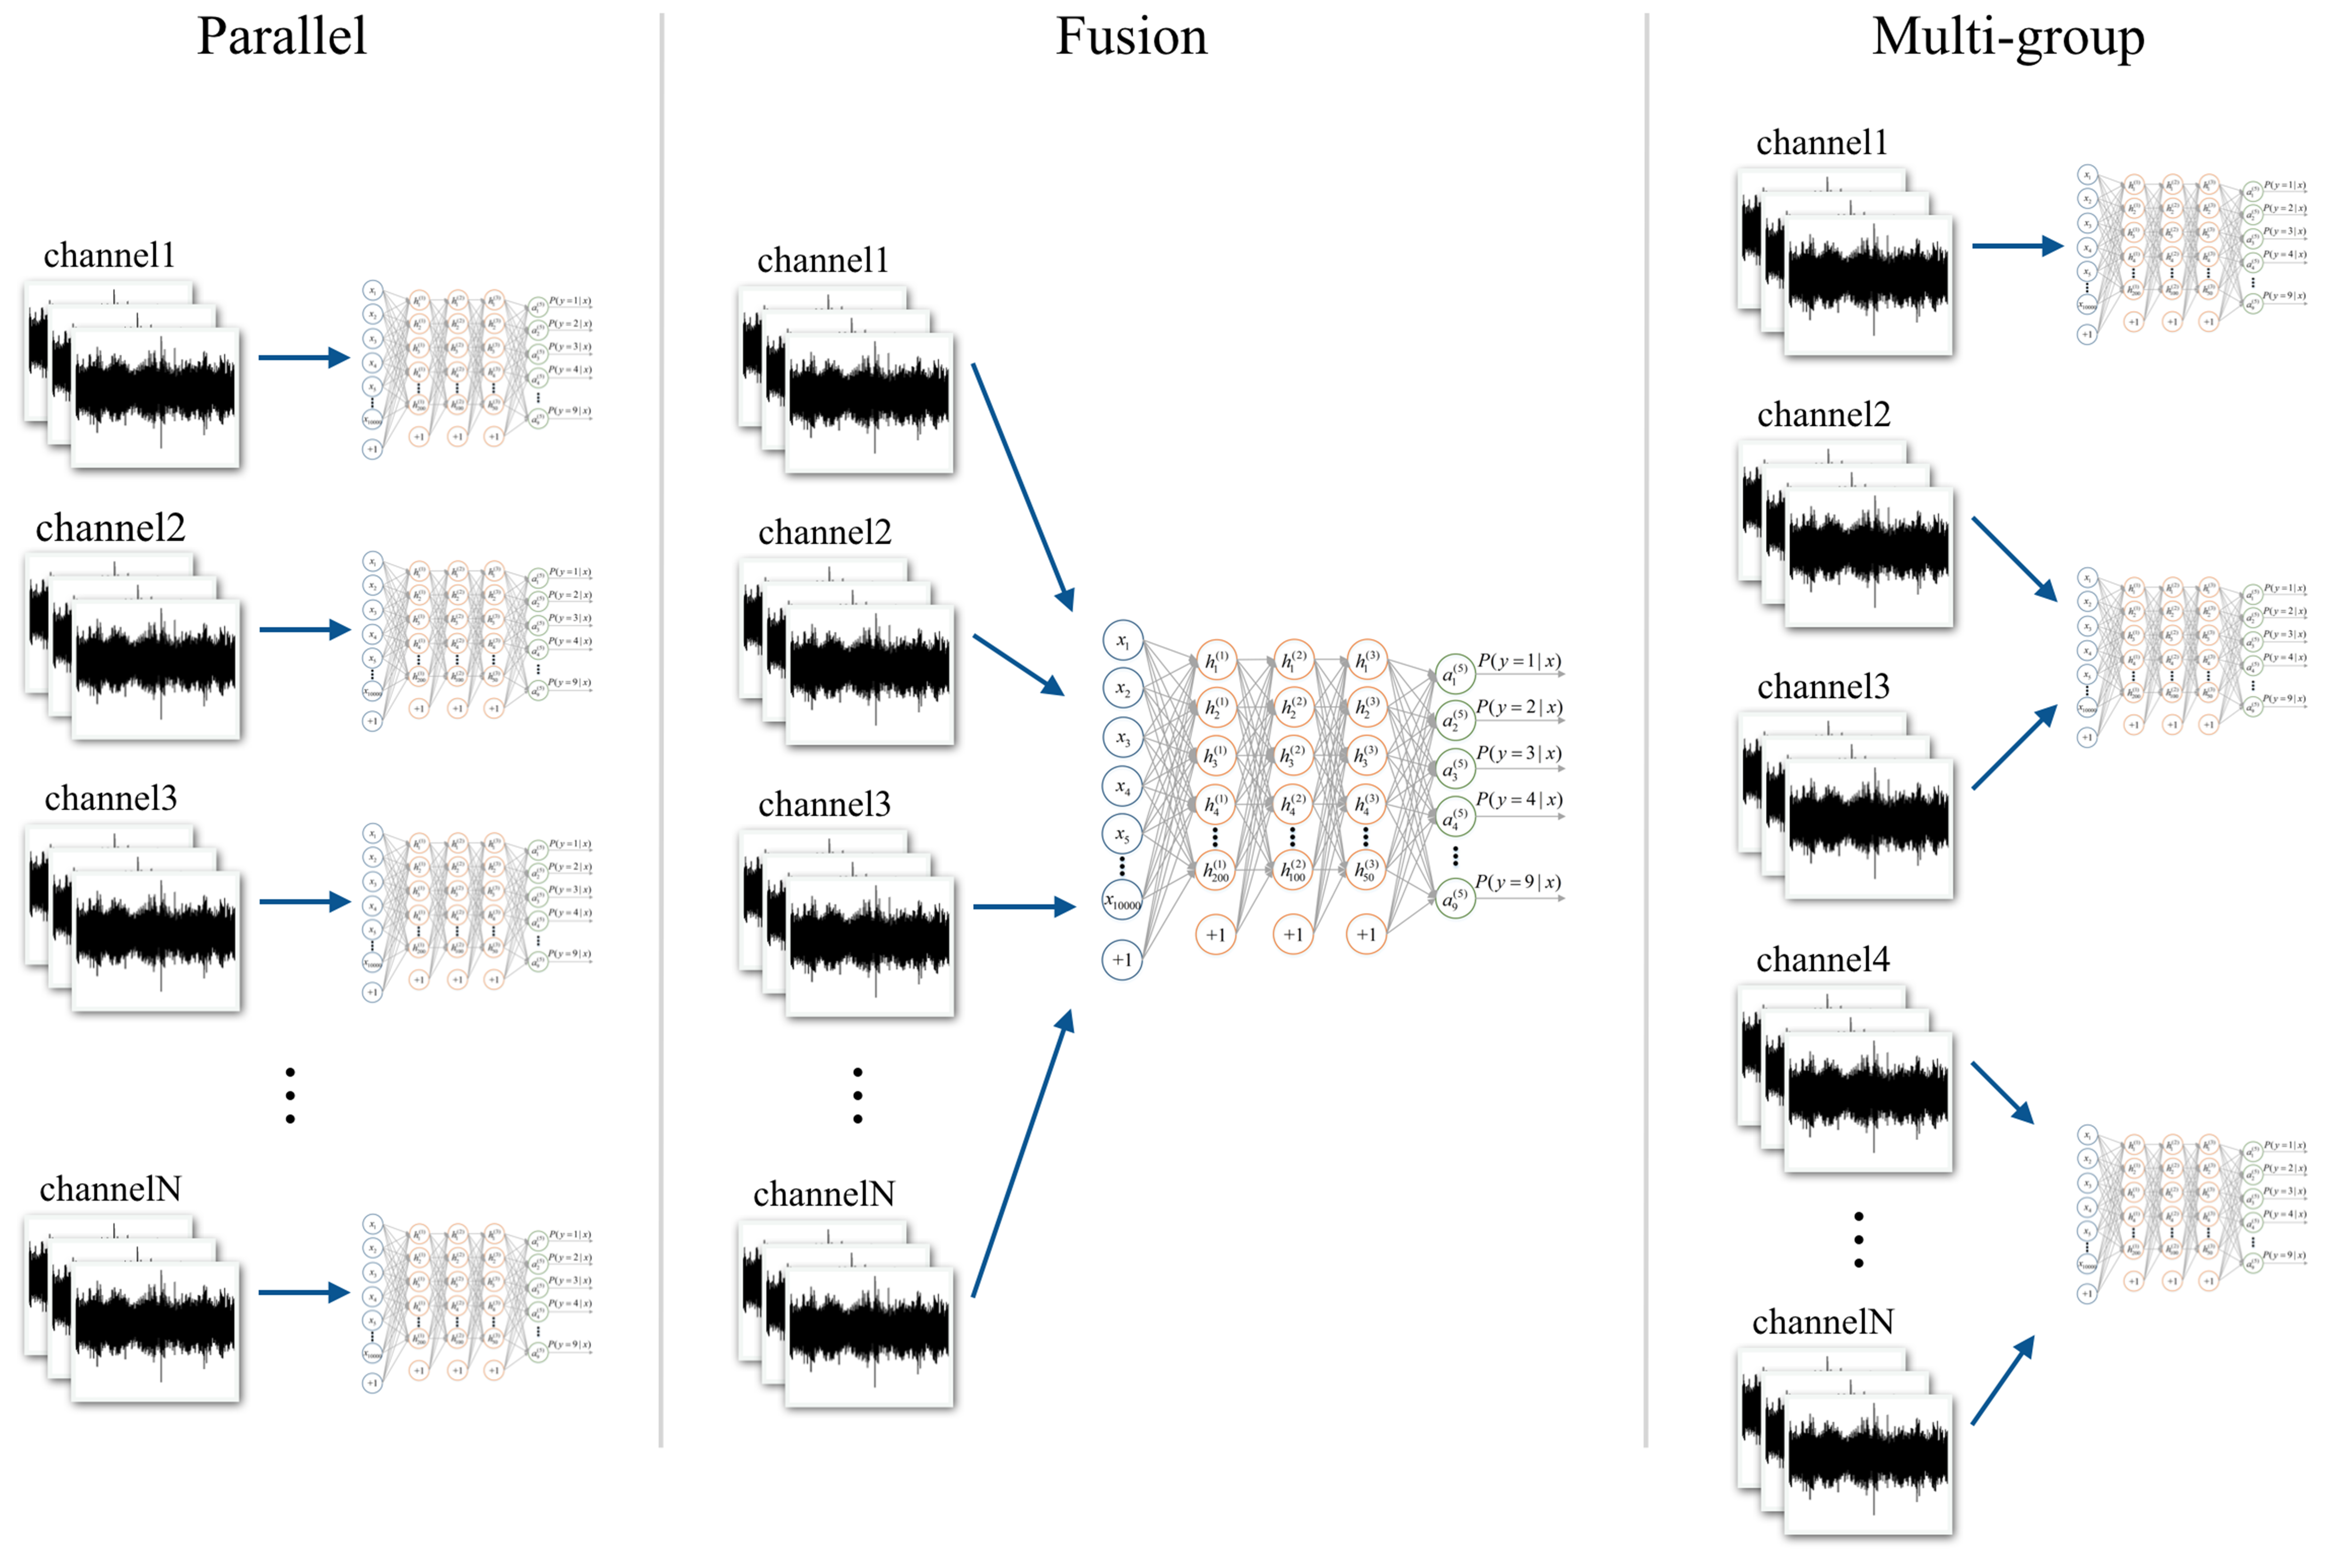
\includegraphics[width=0.9\textwidth]{fig_3-3}
\vspace{0.2em}
\bicaption[Donation]{}{基于计算机视觉和深度学习的异常数据诊断方法框架}{Fig.$\!$}{Framework of the proposed data anomaly detection method}
\end{figure}


\section{大跨度斜拉桥长时距振动监测数据算例验证}[Case study]
\subsection{大跨度斜拉桥结构健康监测系统介绍}[Introduction of the SHM system of a long-span bridge]

作为案例研究,我们考虑中国的一座长跨径斜拉桥(见图4)。该桥主跨1088米,两座边跨各300米,两座306米高的桥塔。自2008年建成以来,该桥的SHM系统包括加速度计、风速计、应变仪、GPS、温度计等。加速度计的信息如图4和表1所示。桥面和桥塔上的加速度计共使用38个通道,其中桥面和桥塔顶部有16个双通道加速度计,桥塔底部有2个三通道加速度计。

在本案例研究中,只考虑SHM系统测得的加速度数据,将加速度数据的异常情况分为六种模式:缺失、微小、离群、平方、趋势和漂移。表2对这六种模式的数据异常特征进行了简要说明。图5为每种模式的典型异常情况。这样的数据异常不仅在加速度数据中常见,在GPS数据、应变数据、风速数据等中也很常见。

\subsection{数据可视化和标记}[Data visualization and labeling]

2012年测得的所有加速数据均绘制在每小时8位灰度图像中,分辨率为100 100像素,共计333792个样本(这里,一个图像就是一个样本)。对于3\%的采样比例,随机选取10014个样本并进行标注,其中50\%生成训练集,另一半作为验证集。作为例子,图6显示了训练集中通道1、2、3各10张图像。请注意,坐标系是不可见的,因为振动响应的持续时间和振幅信息是不需要基于轮廓的分类。图7展示了当样本中存在多异常特征时的5个例子,如2.2节中讨论的那样。

\subsection{DNN设计与训练}[Design and training of DNN]

在这个例子中,桥的SHM系统中传感器的详细信息是未知的。因此,多组DNN布局可能是不可行的。另外,一些数据异常模式在训练数据集中比较少见,容易被遗漏,这将降低训练DNN的数据异常检测精度。采用融合DNN布局,通过共享已标记的数据异常模式来缓解这一问题。

所设计的DNN的架构如图8(a)所示。输入层有10000个节点,因为可视化的图像是一个矢量,其中每个元素都被输入到输入层的一个节点中。输出层有7个节点,分别对应6种模式的数据异常和正常数据。有三个隐藏层,分别有100个、75个、50个节点。每个隐藏层的节点数递减的设计是为了提取较高的抽象特征进行泛化,可以克服随机抽样收集的数据集不平衡导致的过拟合风险。在训练阶段采用了提前停止的方法,图8(b)展示了其性能,表明由交叉熵测量的收敛性在epoch 500时成为最优。图9(a)和9(b)是检查分类结果的混淆矩阵,训练集和验证集的准确率分别为90.7\%和85.8\%。

回收率(最右边一列)是TP数和实际数据集中某个特定模式出现的总次数之比。这个指标评估了分类器从输入事实中获得的可靠性。在训练集和验证集上,"次要 "异常模式的召回率分别只有63.1\%和52.4\%。这种糟糕的表现是因为部分 "次要 "样本被误分类为 "正常",尽管 "正常 "数据的误分类率很低。

精度(混淆矩阵的底行)是预测结果中真阳性(TP)与某类总数的比率。该指标评估了分类器基于输出预测的可靠性。"小 "异常模式的精度高于其召回率,分别达到78.7\%和67.7\%。这一改进是因为来自其他模式的样本被误判为 "次要 "模式的较少。

为了描述的方便,我们用图矩阵来表示特征图。图10说明了所设计的DNN的第一隐藏层中学习的特征。图10中的每个特征图将最大限度地激活第一隐藏层中100个节点中的一个节点,因此公式(5)中的对应输出等于1,有些特征是可以清晰辨认的,如图中 , , , , (表示矩阵中行和列的图),其中的 "趋势 "用 "X "形的交叉线表示。的特点, , , ,学习 "正态 "模式,即水平中间为暗,上下为乱。在 和 中学习 "正方形",边缘清晰。不止一个特征描述了 "次要 "图案,如 , , 和 。"漂移 "与其他层的特征隐性叠加,如在 和 。在 , , ,中的特征会产生明亮的垂直线来代表离群值。最后,在所设计的DNN的第一个隐藏层的特征中没有发现 "缺失 "的模式,虽然这个模式的异常值最多。请注意,"缺失 "模式几乎是空白的纯白色像素,这意味着在第一个隐藏层中没有学习这个模式的特征。不过,"没有特征 "的模式可以通过连续几层的学习步骤中多个特征的叠加来表示。

\subsection{自动异常诊断}[Automatic anomaly detection]


为了测试全训练DNN的数据异常检测能力,采用全年的加速数据。在PC机(CPU:Intel i7-3770,内存:20GB,7200转硬盘)上检测耗时约6小时,与人工检测相比,成本低,省时省力。

图11显示了每个通道中每个数据异常模式的计数。每条的总计数为8784 h,图11中的38个通道大致分为4组:通道1-3、4-12、13-28、29-38。相比较而言,第2组和第4组的数据质量可以接受,7000 h以上的数据都是正常的,大部分异常数据被归为 "缺失 "或 "轻微";第1组和第3组的数据质量较差,6种数据异常模式均占主导地位。计数结果见表3,说明30.08\%的数据为异常数据。而 "轻微 "模式是数据的主要异常形式,占数据总量的10.99\%。

图12显示了2012年的数据异常分布情况。很明显,在空间和时间上出现了几个广泛的集群;这些集群按时间顺序用数字标示。通道1至3构成了集群1,主要由贯穿全年的 "小 "模式组成。注意,集群2包含13~24个通道。如图4所示,这些信道都在大桥主跨的南侧,说明它们很可能在一个子网中,届时这个传感器子系统可能会出现严重的错误。同样,簇3中包含了25-28个通道,这些通道位于大桥南侧边跨,从1月到4月初同时产生了一大块 "方块 "图案。集群4显示,整个SHM系统在4月下旬失效,因为没有一个传感器记录到任何数据。集群5和6由通道5-12中的 "缺失 "图案组成;这些通道位于靠近主跨的北侧。最后,通道13-24均匀地出现故障,产生了与集群2类似的集群7。除了这些群组外,还有零星的异常现象散布在一年中,如图12所示。

数据异常分布与数据异常模式和传感器通道的计数结果分别如图13和图14所示。图13中,"缺失"、"方块"、"趋势"、"漂移 "数据异常模式的分布相对集中,而 "次要"、"离群 "模式在时空上是分散的。图14显示,同组的通道(见图11)不仅总体数据质量相似,而且在异常模式分布和时空趋势上也很相似。以上信息为进一步的数据清洗和分析,以及SHM系统的准确维护提供了指导。此外,所提出的方法还可以大大减少SHM系统中因异常引起的误报次数。

为了验证所提方法的可靠性,对2012年所有图像样本进行人工标注,与所提方法的检测结果进行对比。2012年的实际数据异常分布如图15所示,表明其结果与建议方法得到的图12的检测结果基本一致。实际数据异常的计数结果如表4所示,表明34.09\%的数据存在异常。非常接近于表3所示的检测结果中总数据异常的30.08\%,"小 "模式是数据的主要异常形式,在总数据中占14.92\%。

图16是用于进一步验证所提出方法可靠性的混淆矩阵。对于 "正常 "和 "缺失 "模式,召回率和精度都保持在90\%以上的高值;对于 "小 "模式,42.13\%的 "小 "样本被误判为 "正常",3.43\%的 "正常 "样本被误判为 "小",因此召回率和精度都低于其他模式的;"离群 "模式的召回率和精度适中,分别为74. 0\%和70.6\%;对于 "方块 "模式,实际 "方块 "样本中有76.9\%被正确检测出来,检测结果中93.1\%为真阳性,是可以接受的;"趋势 "模式的召回率和精度较好,分别达到88.6\%和84.5\%,由于 "漂移 "模式量少,精度被其他模式的误分类样本拖累到47.9\%。最后,一年测试数据的总准确率为87.0\%,说明所提出的方法具有良好的SHM数据异常检测能力。

\section{讨论与结果}[Discussion and conclusion]

本文提出了一种基于计算机视觉和深度学习的数据异常检测方法,以自动检测SHM系统中的异常。通过模仿人类专家,首先将SHM时间序列数据转换成图像,供计算机可视化,然后将灰度数字的图像向量作为DNN的训练集。设计好DNN后,采用贪婪的分层训练技术对其进行训练。采用SHM系统对某长跨径斜拉桥的测得的加速度数据来验证所设计和训练的DNN的可行性和准确性。示例中使用的数据包含6种数据异常模式,设计和训练的DNN对数据异常检测结果的全局准确率可以达到87.\%。得到的数据异常分布和传感器侧的异常计数结果,对进一步精确的数据清洗和SHM系统的维护很有帮助。与人工检测方法相比,提出的基于计算机视觉和深度学习的方法效率更高。

所提出的方法为SHM数据预处理提供了一个新的视角,对于SHM系统的自动实时监测和报警,以及基于数据的结构物离线长期性能分析都是必不可少的。虽然本文只关注加速度数据,但也可以应用于其他类型的传感器数据。在今后的工作中,应更多地关注异常点图像的无监督学习表示,以减少人工干预。此外,对于SHM系统测量数据中的并发异常,可以采用多标签分类方法。


% Local Variables:
% TeX-master: "../main"
% TeX-engine: xetex
% End: